\setlength{\footskip}{8mm}

\chapter{Literature Review} 
\label{ch:literature-review}

This chapter describes the literature review on the algorithms in
several key parts for behavior understanding and anomaly detection,
and the real-world open source and commercial video surveillance
products.

\section{Algorithms}

Human behavior understanding and anomaly detection problem becomes
more challenging in the area of computer vision. It can be divided
into three main key parts: behavior representation and tracking,
behavior clustering, and behavior modeling and anomaly detection.

%Finally, we also add the literature on incremental learning, which is
%a growing area and also has received many research attentions in the
%computer vision and machine learning community these days in order to
%improve real-time surveillance systems.

\subsection{Behavior Representation and Tracking}

Behavior representation is the first key step in human behavior
understanding. In this section, we review the existing algorithms 
for blob extraction, shadow detection and removal, and tracking.

\subsubsection{Blob Extraction}
\label{literature-review-blob-extraction}

To extract blobs or foreground objects from a scene, image processing
techniques are required here. There are many techniques that can be
applied for this task. The most simple one is image
differencing. \shortciteA{yamato92hmm} apply this technique to extract
blobs or human from a scene by the following conditions:
\[
\begin{array}{lc}
  {\rm if} & \left|{I_a (x,y) - I_b (x,y)}\right|< T,\;I_e (x,y) = 0 \\ 
  {\rm else} & I_e (x,y) = I_a (x,y), 
\end{array}
\]
where $I_e (x,y)$ is a human extracted image, $I_a (x,y)$ is an
original image, $I_b (x,y)$ is a background image, and $T$ is a
threshold. The authors binarize the extracted image to calculate the
mesh feature. Mesh features have been used as the low-level image
features, and also have been successfully applied to complex 2D
patterns such as multi-font characters \shortcite{umeda82font}. The
calculation of mesh features is shown in Figure
\ref{fig:mesh-feature}. The ratio of black pixels to total pixels in
each mesh is an element of the feature vector.

\begin{figure}[t]
  \centering
  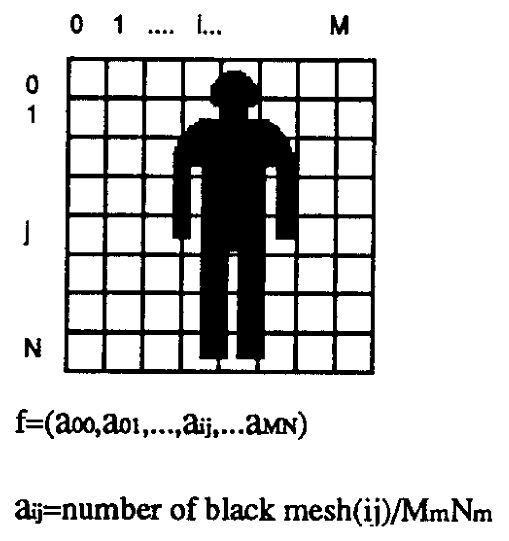
\includegraphics[width=2in]{figures/mesh-feature.jpg}  
  \caption[Mesh feature calculation]{Mesh feature
    calculation. Reprinted from the work of Yamato et al.\ (1992).}
  \label{fig:mesh-feature}
\end{figure}

\shortciteA{nair02surveillance} slightly improve the image differencing 
technique by updating the background model and threshold for every
frame using temporal averaging. They first model the background by
taking the average of five consecutive frames without anyone in the
scene. The labeled pixels are considered as foreground when they
satisfy the following condition:
\[
  \left|{I_n (x,y) - B_n (x,y)}\right| > T_n (x,y),
\]
where $I_n (x,y)$ is the current frame, $B_n (x,y)$ is the current
background model, and $T_n (x,y)$ is a threshold function. The authors
initialize the threshold value to 50 at all pixel locations. The
background model and threshold function are then updated using
temporal averaging as follows:
\[
B_{n + 1} (x,y) = \left\{ 
\begin{array}{l}
  B_n (x,y) \\ 
  \alpha B_n (x,y) + (1 - \alpha )I_n (x,y) \\ 
\end{array} \right.
\begin{array}{*{20}c}
  {{\rm if}\;(x,y)\;{\rm is}\;{\rm foreground},} \hfill  \\
  {{\rm otherwise}} \hfill  \\
\end{array}
\]
\[
T_{n + 1} (x,y) = \left\{ 
\begin{array}{l}
  T_n (x,y) \\ 
  \alpha T_n (x,y) + 2(1 - \alpha )\left| {I_n (x,y) - B_n (x,y)} \right| \\ 
\end{array} \right.
\begin{array}{*{20}c}
  {{\rm if}\;(x,y)\;{\rm is}\;{\rm foreground},} \hfill  \\
  {{\rm otherwise}}, \hfill  \\
\end{array}
\]
where $\alpha$ is a constant to determine how fast $B_n (x,y)$ and
$T_n (x,y)$ adapt to changes. In this paper, the authors use the
coordinates of the blob's center of mass, average color, and height to
represent a blob.

Although the image differencing technique is fast and commonly used in
many surveillance applications such as
ZoneMinder \shortcite{zoneminder}, it is very sensitive to noise, and
also cannot deal with most of the cluttered background scenes.

There are many researchers who try to improve the background modeling
for cluttered scenes and utilize the color information to classify a
pixel whether it is foreground or
background. \shortciteA{wren97pfinder} first propose to model a
background scene using a single Gaussian distribution per pixel in the
YUV color space. Each pixel is represented by a vector $[Y, U,
V]^T$. The authors define some threshold to classify whether a pixel
is foreground or background. If the log likelihood is smaller than the
threshold, the pixel is considered as foreground; otherwise, it is
considered as background. Using this background modeling technique
with the proper parameters will yield reasonable results for both
indoor and outdoor scenes. Although this technique can deal with
noise, it has the problem with gradual illumination change and is
still unsuitable for some cluttered background scenes.

One of the well-known background modeling techniques is that
of \shortciteA{stauffer99background} who propose a method that models
multi-modal background distributions using a mixture of Gaussian (MoG)
distribution. This technique performs better than the single Gaussian
background modeling since multi-modal background distributions occur
more frequently in outdoor scenes. The authors first model the recent
history of each pixel using a mixture of $K$ Gaussian
distributions. $K$ is determined by the available memory and
computational power. They then classify pixel values that do not fit
one of the background distributions as foreground until there is a
Gaussian distribution that supports those
values. Figure \ref{fig:bck-model-results} shows the results from
using the single and MoG background modeling\nocite{anh08thesis}.

\begin{figure}[t]
  \centering
  \subfloat[]{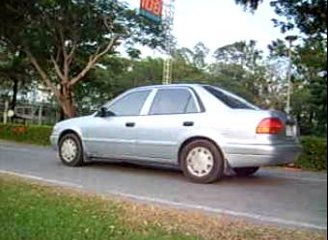
\includegraphics[scale=0.5]{figures/car-original.jpg}
  \label{fig:car-original}}
  \hspace{0.1in}
  \subfloat[]{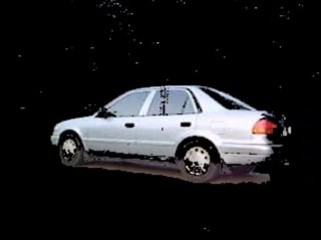
\includegraphics[scale=0.5]{figures/car-sgm-result.jpg}
  \label{fig:car-sgm-result}}
  \hspace{0.1in}
  \subfloat[]{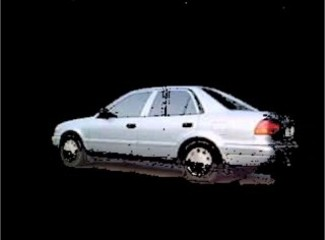
\includegraphics[scale=0.5]{figures/car-mog-result.jpg}
  \label{fig:car-mog-result}}
  \caption[Example of single and MoG background modeling results.]
  {Example of single and MoG background modeling results. (a) Original
  image. (b) Foreground pixels using the single Gaussian background
  modeling. (c) Foreground pixels using the MoG background
  modeling. Reprinted from the work of Tuan Anh (2008).}
  \label{fig:bck-model-results}
\end{figure}

However, the MoG background modeling still faces a problem to deal
with gradual illumination changes. In order to solve this
problem, \shortciteA{poppe07background} modify the matching step of
the MoG background modeling. Their idea is to store the previous pixel
value and previous matching model number, and use them in the matching
step. In this step, each pixel is checked with the $K$ Gaussian
distributions. For the model which matches the pixel in the previous
frame, the difference between the current pixel value and previous
pixel value is small enough for some threshold, a match is
intermediately defined; otherwise, the normal matching step is
followed. If the matched model represents the background, the model
number and the current pixel value are stored; otherwise, they retain
their values. By following this way, foreground objects will not
affect the recent history. Figure \ref{fig:poppe-bck-model-results}
shows the results from using the MoG background modeling and the
improved MoG background modeling.

\begin{figure}[t]
  \centering
  \subfloat[]{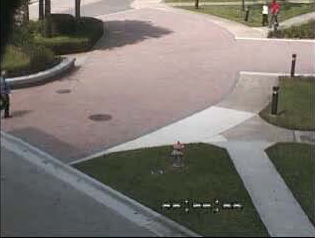
\includegraphics[scale=0.5]{figures/poppe-original.png}
  \label{fig:poppe-original}}
  \hspace{0.1in}
  \subfloat[]{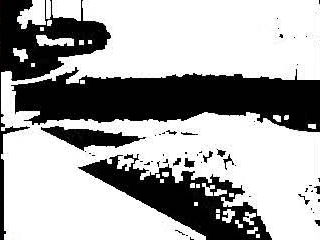
\includegraphics[scale=0.5]{figures/poppe-mog-result.png}
  \label{fig:poppe-mog-result}}
  \hspace{0.1in}
  \subfloat[]{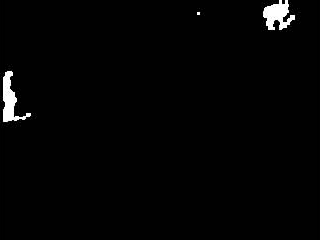
\includegraphics[scale=0.5]{figures/poppe-improved-mog-result.png}
  \label{fig:poppe-improved-mog-result}}
  \caption[Example of MoG and improved MoG background modeling
  results.]{Example of MoG and improved MoG background modeling
  results. (a) Original image. (b) Foreground pixels using the MoG
  background modeling. (c) Foreground pixels using the improved MoG
  background modeling. Reprinted from the work of Poppe et al.\
  (2007).}
  \label{fig:poppe-bck-model-results}
\end{figure}

Although a lot of work has tried to improve the classic background
modeling techniques, the fragmentation problem caused by a cluttered
background still exist in blob detection and segmentation
process. This problem is unavoidable in practice;
therefore, \shortciteA{lu08segmentation} attempt to solve this problem
and propose an effective connected components labeling method called
connected chips linking (CCL). In this paper, they provide a function
to calculate the correlation of space location between two blobs. Then
they construct a correlation matrix based on the result. In order to
handle fragmented blobs, they cluster the blobs using the information
from the correlation matrix through the mean-shift algorithm. After
that, they classify the blob-sets into ``Human'' or ``Fragments''
using some criteria such as human
size. Figure \ref{fig:blob-clustering-result} shows the result of
handling fragmented blobs.

\begin{figure}[t]
  \centering
  \subfloat[]{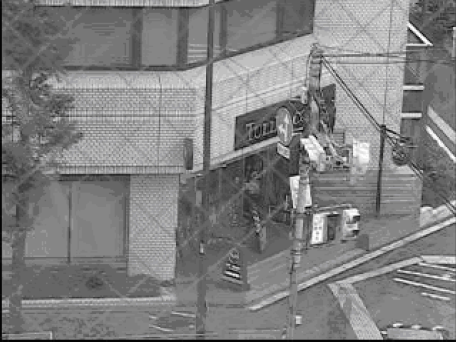
\includegraphics[scale=0.3]{figures/blob-clustering01.png}
  \label{fig:blob-clustering01}}
  \hspace{0.01in}
  \subfloat[]{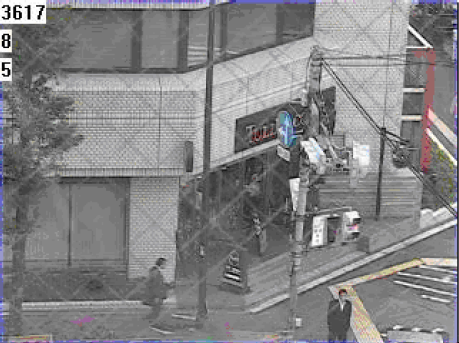
\includegraphics[scale=0.3]{figures/blob-clustering02.png}
  \label{fig:blob-clustering02}}
  \hspace{0.01in}
  \subfloat[]{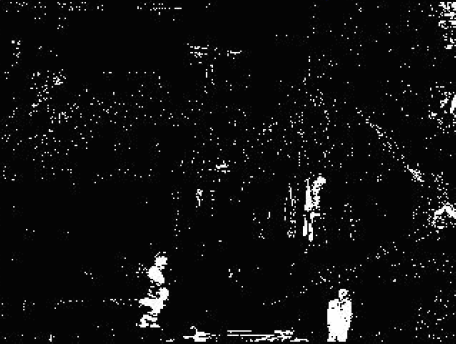
\includegraphics[scale=0.3]{figures/blob-clustering03.png}
  \label{fig:blob-clustering03}}
  \hspace{0.01in}
  \subfloat[]{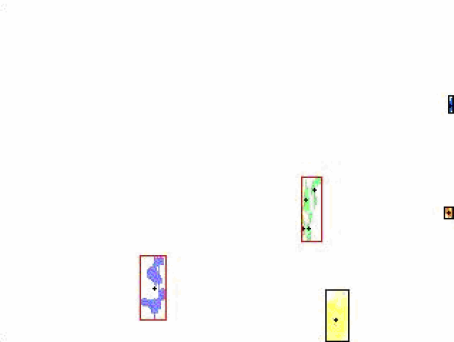
\includegraphics[scale=0.3]{figures/blob-clustering04.png}
  \label{fig:blob-clustering04}}
  \caption[Example of the result of handling fragmented
  blobs.]{Example of the result of handling fragmented blobs. (a)
  Background image. (b) Current image. (c) Foreground pixels. (d)
  Result of handling fragmented blobs. Reprinted from the work of Lu
  et al.\ (2008).}
  \label{fig:blob-clustering-result}
\end{figure}

After segmenting the blob, the next step is to extract the blob
features. \shortciteA{li06behavior} use the least median of squares
(LMedS) method to construct the background model, then extract
foreground by subtracting the background image. The authors propose a
method based on space-time image features for automatic behavior
modeling and recognition. This method is simple and insensitive to
noise, and does not need to track parts of the human body. In this
method, they extract the foreground, calculat shape features,
represent the features as a space-time image. After the foreground is
extracted, the authors equidistantly divide the bounded rectangle of
the foreground into $10\times7$ sub-blocks. Then they normalized the
value of each sub-block as follows:
\[
d_i = \left\lfloor {\frac{{s_i}}{{M}}\times255} \right\rfloor, i =
  1,2, \ldots,k,
\]
where $k=10\times7$ is the number of sub-blocks; $s_i$ is the number
of the foreground pixels in the $i^{th}$ sub-block; $M$ is the maximum
value of $s_i$, where $i=1,2,...,k$. After that, they have the
resulting shape descriptor $D_t$ at image frame $t$: $D_t =
[d_1,d_2,d_3,...,d_k]$. Finally, to represent the motion of a sequence
with $t$ frames, they construct the space time image representation
(see Figure \ref{fig:space-time-feature}) as a matrix $I$ of size
$t\times k$ as:
\[
I = [D_1,D_2,D_3,...,D_t]^{T}_{t\times k}
\]
They extract the features from this representation by Gabor filtering as 
follows:
\[
F_n (x,y) = \iint {I_n (x_1 ,y_1 )G(x - x_1 ,y - y_1 ,f)dx_1dy_1},
\]
\[
G(x,y,f) = \frac{1}{{2\pi \sigma _x \sigma _y }}\exp \left[ {
- \frac{1}{2}\left( {\frac{{x^2 }}{{\sigma _x^2 }} + \frac{{y^2
}}{{\sigma _y^2 }}} \right)} \right]M(x,y,f),
\]
\[
M(x,y,f) = \cos \left[ {2\pi f(x\cos \theta + y\sin \theta)} \right],
\]
where $I_n(x,y)$ is the $n^{th}$ space-time image; $F_n(x,y)$ is the filtered 
space-time image; the space constants of the Gaussian envelope along the $x$ 
and $y$ axis are represented by $\delta _x$ and $\delta _y$, respectively; $f$ 
is the frequency of the sinusoid and $\theta$ is the orientation of the Gabor 
filter.

\begin{figure}[t]
  \centering
  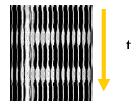
\includegraphics[width=1.5in]{figures/space-time-feature.jpg}
  \caption[Space-time image representation]{Space-time image
  representation. Reprinted from the work of Li et al.\ (2006)}
  \label{fig:space-time-feature}
\end{figure}

There are some feature extraction methods that are able to capture
motion history rather than having only current static
features \shortcite{yamato92hmm,nair02surveillance}. One of them is
motion history image (MHI) \shortcite{davis97mhi}. MHI is a static
image template where pixel intensity is a function of the recency of
motion in a video sequence. The idea is to represent how motion the
image is moving. The MHI is defined as:
\[
  H_\tau  (x,y,t) = \left\{ \begin{array}{l}
  \tau \quad \quad \quad \quad \quad \quad \quad \quad \quad \quad \quad \quad 
  {\rm if}\;D(x,y,t) = 1 \\ 
  \max (0,H_\tau  (x,y,t - 1) - 1)\quad {\rm otherwise}, \\ 
  \end{array} \right.
\]
where $H_\tau (x,y,t)$ represents the MHI for a pixel $(x,y)$ at time
$t$. The more recently moving pixels will be
brighter. Figure \ref{fig:mhi} presents the examples of MHIs.

\begin{figure}[t]
  \centering
  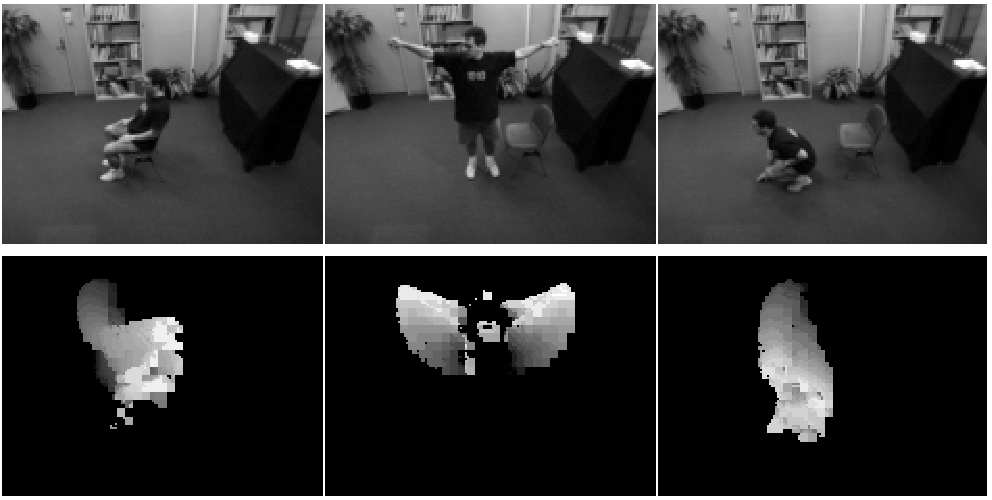
\includegraphics[width=4in]{figures/mhi}
  \caption[Examples of motion history images]{Examples of motion
  history images. Reprinted from the work of J. Davis \& Bobick
  (1997).}
  \label{fig:mhi}
\end{figure}

Based on the local intensity history of
pixels, \shortciteA{xiang02event} proposed the pixel change history
(PCH) to characterize pixel-wise temporal visual information in order
to detect pixel-level events. The PCH is a representation of
pixel-wise changes based on a combination of the pixel signal energy
(PSE) proposed by \shortciteA{ng03pixel} and the MHI, which is
computed as follows:
\[
  P_{\varsigma ,\tau } (x,y,t) = \left\{ \begin{array}{l}
  \min (P_{\varsigma ,\tau } (x,y,t - 1) + \frac{{255}}{\varsigma },255)\quad 
  \; {\rm if}\;D(x,y,t) = 1 \\ 
  \max (P_{\varsigma ,\tau } (x,y,t - 1) + \frac{{255}}{\tau },0)\quad \quad 
  {\rm otherwise}, \\ 
  \end{array} \right.
\]
where $P_{\varsigma ,\tau } (x,y,t)$ represents the PCH for a pixel
$(x,y)$ at time $t$, $D(x,y,t)$ indicates foreground regions at time
$t$, $\varsigma$ is an accumulation factor, and $\tau$ is a decay
factor. When the accumulation factor is set to 1, the PCH over the
entire image is equivalent to the MHI. In this work, they did not
specifically recognize human behaviors, but they proposed a new
low-level primitive applicable to human representation that can
describe human actions efficiently.

Recursive filtering \shortcite{masoud03recognition} is a technique
that encodes motion information such as the speed of the motion within
a short period of time. The idea is to represent the ``recency'' of the
motion. This technique is conceptually similar to the MHI. Let $I_t$
be the frame at time $t$ and the filtered image $F_t$ at time $t$ is
defined as follows:
\[
  F_t = \left| {I_t  - M_t } \right|
\]
\[
  M_t = (1 - \beta)M_{t - 1}  + \beta M_t 
\]
\[
  M_0 = I_0 = {\rm Background},
\]
where $t = 1, 2, \cdots, n_i$. If $\beta = 0$, the filtered image
$F_t$ will be the foreground and if $\beta = 1$, $F_t$ will be
equivalent to image differencing. Examples of filtered images are
presented in \figurename~\ref{fig:f-img}.

\begin{figure}[t]
  \centering
  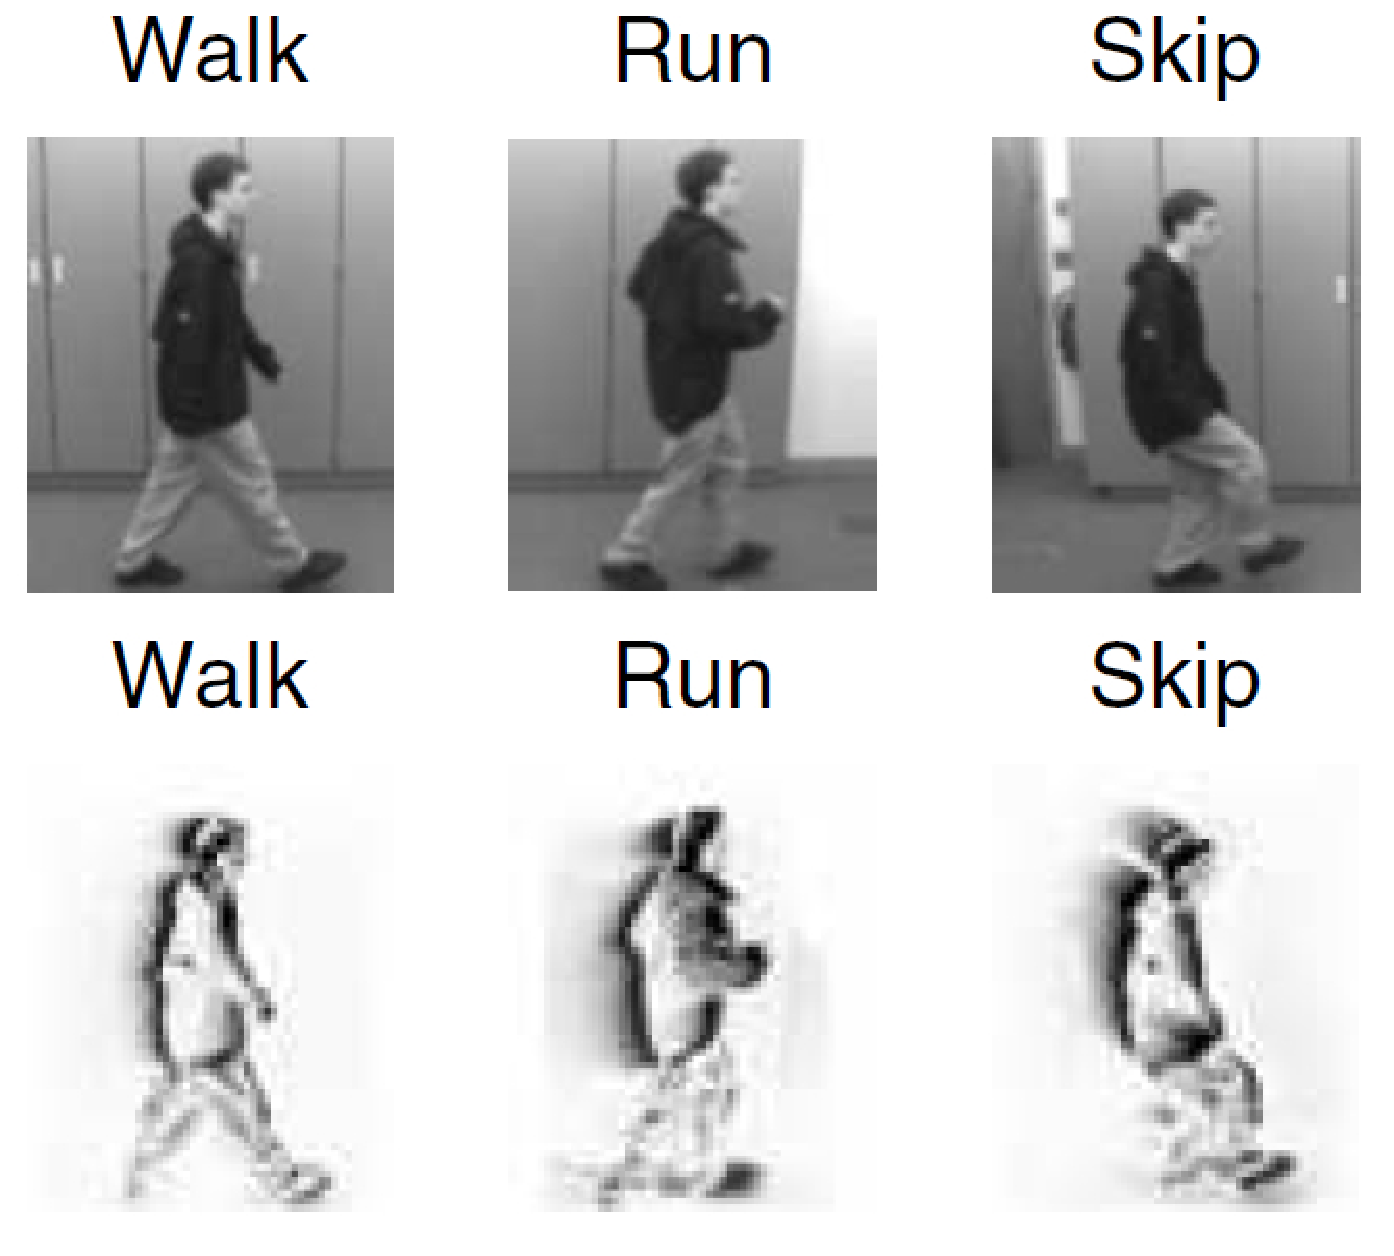
\includegraphics[width=2.5in]{figures/f-img}
  \caption[Examples of filtered images]{Examples of filtered
  images. The coefficient $\beta$ is set to 0.5. Reprinted from the
  work of Masoud \& Papanikolopoulos (2003).}
  \label{fig:f-img}
\end{figure}

\subsubsection{Tracking} 

Tracking people in a scene is a very difficult problem and it is one
of the most active research fields in computer vision. Due to
occlusion ambiguity, the task of tracking and distinguishing each
person is more challenging. In video surveillance applications, it is
necessary to track moving objects or people passing in a scene in
real-time. Moreover, tracking human can be considered as a step before
modeling human behaviors. One of the most well-known techniques for
multiple human tracking is the Kalman
filter \shortcite{kalman60filtering}. The Kalman filter also has been
extensively applied for tracking in many domains.

In visual surveillance, \shortciteA{niu03tracking} propose a method to
use a second order Kalman filter to track each person individually,
and to handle occlusion problems. They define a state including
position, velocity, and acceleration. When a new person is detected,
they store a unique label for that person having the information:
height, centroid, and the average intensity value of the region of the
person. Then they use this information to continue keeping track of
the person in each frame.

\shortciteA{bodor03recognition} develop an automated system to track
individual pedestrians, and alarm the security personnel when a
pedestrian enters a secure area. In this paper, they track each
pedestrian through the development of a position and velocity path
characteristic using a Kalman filter. The limitations of the paper are
that the system yields some errors when there are significant changes
in lighting, and it also cannot distinguish between pedestrians moving
at the same speed.

\shortciteA{girondel04tracking} also propose a method for multiple
human tracking using the Kalman filter to solve the occlusion
problems. They define a Kalman filter for each person, then predict
the person's bounding box, the face's boding box, and the speed. They
use a state vector of ten components for each Kalman filter: the
corners of the bounding boxes of the person and face plus two
components for face speed. For the face detection, they use skin
detection to detect face and hands, and assume that face is a bigger
blob, and moves more steadily. In this paper, they use the combination
of a forward tracking phase and a backward tracking phase to track
between detected objects on two consecutive frames. This technique is
also called ``forward and backward overlapping'' which will be
hereinafter described in more details in my methodology. An example of
tracking results of this method is shown
in \figurename~\ref{fig:girondel-tracking-result}.

\begin{figure}[t]
  \centering
  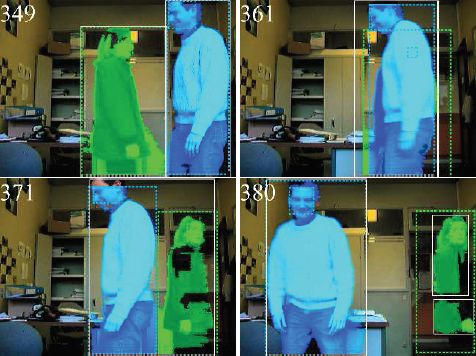
\includegraphics[width=2in]{figures/girondel-tracking-result.png}
  \caption[Example of tracking results of Girondel et al.'s
  method]{Example of tracking results of Girondel et al.'s
  method. Reprinted from the work of Girondel et al.\ (2004).}
  \label{fig:girondel-tracking-result}
\end{figure}

\shortciteA{rosales99tracking} propose a method for tracking
multiple persons in a 3D space. They assume that the system is
observing multiple moving persons via a single uncalibrated video
camera. Therefore, an extended Kalman filter (EKF) formulation is used
to estimate the relative 3D motion trajectories up to a scale
factor. The authors select only two feature points which are two
opposite corners of the person's bounding box to reduce the complexity
of the tracking problem. The 3D size of the person's bounding box is
assumed to remain approximately the same, or at least vary
smoothly. They consider the persons as being planar; therefore, the
depth at both feature points would be the same. Their state vector
then become:
\[
  \vec{x} = (x_0 ,y_0 ,x_1 ,y_1 ,z\beta ,\dot x_0 ,\dot y_0
  ,\dot x_1 ,\dot y_1 ,\dot z\beta )^T,
\]
where $(x_0, y_0, z\beta)^T$, $(x_1, y_1, z\beta)^T$ are the corners
of the 3D planar bounding box and $(\dot x, \dot y, \dot z\beta)^T$
represents a corner's 3D velocity relative to the camera. Their
experiments demonstrate that their proposed method using 3D trajectory
estimation significantly improves the robustness over methods using 2D
trajectory estimation. An example of 3D tracking result of this method
is shown in \figurename~\ref{fig:rosales-tracking-result}.

\begin{figure}[t]
  \centering
  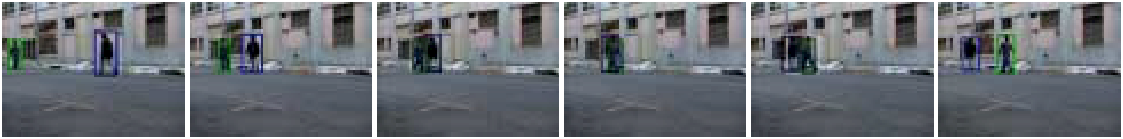
\includegraphics[width=6in]{figures/rosales-tracking-result.png}
  \caption[Example of 3D tracking results]{Example of 3D tracking
  results. Two persons walking in different trajectories, and then
  occluding each other. Reprinted from the work of Rosales and
  Sclaroff (1999).}
  \label{fig:rosales-tracking-result}
\end{figure}

\shortciteA{senior06tracking} solve the occlusion problems by
modeling moving objects using an appearance model. The authors use the
model to localize objects during partial occlusions, detect complete
occlusions, and resolve depth ordering of objects during
occlusions. In this paper, they use a RGB color model to be the
appearance model with an associated probability mask for each
foreground blob. The appearance model of each blob is then updated on
subsequent frames. They also construct a distance matrix by a bounding
box distance measure. Then they use it to determine the association
between tracks and foreground blobs. This technique is similar to the
forward and backward overlapping. In this paper, they evaluated the
proposed method using the PETS 2001 data set 1, camera 1. The results
show that their algorithm successfully copes with complex real world
interactions.

\subsection{Human Behavior Clustering}

More recently, research has started to focus on unsupervised analysis
and clustering of behaviors in a particular scene for a variety of
purposes including anomaly detection, surveillance, and
classification.

\shortciteA{zhong04detection} propose an unsupervised method for
detecting unusual activity in a video. They treat video segments as
documents and clustered the documents based on the co-occurrence
information. Complex activity models and supervised feature selection
are not required in this paper.

\shortciteA{xiang05profiling} model the distribution of activity
data in a scene using a Gaussian mixture model (GMM). Additionally,
the authors also employ the Bayesian information criterion
(BIC) \shortcite{schwarz78bic} to select the optimal number of
behavior classes prior to the training process of hidden Markov models
(HMMs).

\shortciteA{li06behavior} cluster human gestures by constructing an
affinity matrix using dynamic time warping
(DTW) \shortcite{sakoe78dtw,chu02dtw}, then they apply the
normalized-cut approach to cluster the gestures.

\shortciteA{hautamaki08clustering} propose a time-series clustering method. 
In this paper, they apply DTW, and use the pairwise DTW distances as
input to a clustering process in which $k$-means is used to fine-tune
the output of hierarchical clustering.

\shortciteA{swears08clustering} propose hierarchical HMM-based
clustering to find and cluster motion trajectories and velocities in a
highway interchange scene. They build up a set of HMMs
incrementally. For each new trajectory, they first test the likelihood
of the trajectory according to each existing HMM model. If the new
observation is not fit by any existing model, it is considered deviant
and is grouped with other deviant observations to form a new HMM. An
example of the clustering results is shown
in \figurename~\ref{fig:swears-clustering-result}.

\begin{figure}[t]
  \centering
  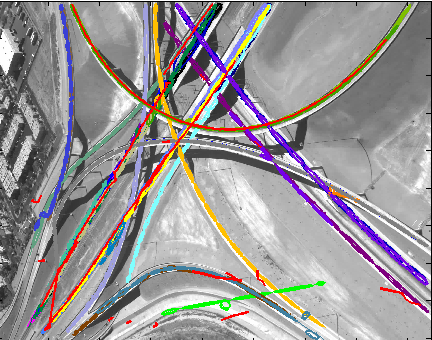
\includegraphics[width=3in]{figures/swears-clustering-result.png}
  \caption[Example of clustering tracking results]{Example of
    clustering tracking results. Overlaid tracks are color coded with
    their HMM assignment. Red tracks indicate positional or velocity
    deviations. Reprinted from the work of Swears et al.\ (2008).}
  \label{fig:swears-clustering-result}
\end{figure}

\shortciteA{alon03clustering} propose a method to discover groupings
of similar object motions. They apply a finite mixture of HMMs where
the number of mixture components is assumed to be known. They estimate
the number of clusters using the minimum description length (MDL)
criterion \shortcite{rissanen98mdl}, a penalized likelihood measure.

\shortciteA{oates01clustering}, who first propose the idea of using
the DTW with HMMs to cluster time series. Their method uses the DTW
dendrogram cut off at an arbitrary depth as an initial partition of
the training sequences, then they train HMMs on each partition in an
iterative fashion until they have a set of HMMs that models all of the
training sequences. They apply their method to simulated time series
with good results, but report obtaining poor clustering resulted in an
experiment with real robot sensor data.

\shortciteA{li99pattern} use the BIC for HMM model selection and
constructed a binary hierarchical clustering dendrogram to initialize
data partitions based on a sequence-to-model likelihood distance
measure. They then compare each pair of clusters using a partition
mutual information (PMI) criterion \shortcite{bahl86speech} to find
the optimal number of clusters.

\subsection{Human Behavior Modeling and Anomaly Detection}

Human behavior understanding is an important component of a wide
variety of desirable intelligent systems. However, the problem is very
difficult, due to the wide range of activities possible in any given
context and the large amount of variability within any particular
activity. The goal of behavior profiling and abnormality detection is
to learn a model which is capable of recognizing expected normal
behaviors as well as detecting abnormal behaviors.

As video monitoring is becoming more ubiquitous in our lives, research
on advanced surveillance video analysis techniques is increasingly
important. To make the work of security personnel reliable and
efficient, normal or typical events need to be filtered out, and in
cases of unusual or abnormal events, an alarm needs to automatically
be raised. An anomalous event also needs to be presented to a human
operator for consideration as a security threat.

Nowadays there are many algorithms which are capable of modeling
normal human behaviors, and discriminating abnormality from typical
behaviors in a scene.  One of the potential algorithms is hidden
Markov model (HMM). HMM is very well-known, and widely used in speech
recognition. Moreover, HMM has proven itself that it is highly
effective to dealing with sequential data.

\shortciteA{yamato92hmm} apply HMMs to recognize tennis
strokes. They extract features based on the bottom-up approach which
is called mesh feature extraction. The calculation of mesh features is
previously described in
Section \ref{literature-review-blob-extraction}. The mesh features are
converted into symbols using vector quantization since discrete HMMs
are applied in this paper. Then the authors train a separate HMM for
each tennis action. The correct action will yield the highest
log-likelihood given the trained model.

\shortciteA{gao04dining} apply HMMs to recognize dining activity in
a nursing home. For feature extraction, they develop a motion
segmentation algorithm based on dense optical flow and random sample
consensus (RANSAC) to extract motion features. They estimate the
distances between patients' head and their hands. To find the faces,
they use a face detection algorithm from the work
of \shortciteA{schneiderman00detection}. In this paper, they do not
apply the vector quantization, but use continuous HMMs to model
continuous observations. They define four states topology to describe
stages in dining activities. Two states are used for the start and end
of each instance of eating. The third state is used to model motions
from when people perform some gestures. The last state is defined as
``don't care" which models instances when no
motion. Figure \ref{fig:gao-hmm-topology} presents the topology of the
HMM model. Lastly, the authors identify instances of eating using the
trained HMM.

\begin{figure}[t]
  \centering
  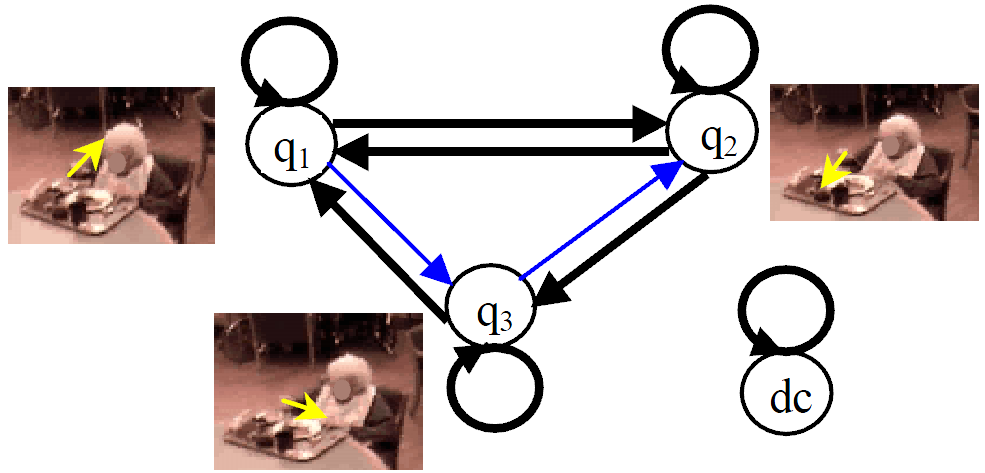
\includegraphics[width=3.5in]{figures/gao-hmm-topology.png} 
  \caption[Topology of the HMM model for dining activity]{Topology of
  the HMM model for dining activity. Reprinted from the work of Gao et
  al.\ (2004).}
 \label{fig:gao-hmm-topology}
\end{figure}

\shortciteA{nair02surveillance} build a video surveillance
application, and also apply HMMs to recognize human behaviors. Their
work is not only to recognize behaviors, but also to detect suspicious
behavior in a corridor scene. They extract simple blob features, which
are center of mass, average color, and height, in the first step of
recognizing human activities. They apply the image differencing
technique as described in
Section \ref{literature-review-blob-extraction}. Then the detected
foreground pixels are grouped by using the connected components
algorithm, and the authors generate a list of blobs detected in the
current frame. They ignore the blobs not matching a the human's
typical aspect ratio. After that, they quantize the feature data into
discrete symbols. Finally, they train a separate discrete HMM for each
activity. A sequence is classified as anomalous if the log likelihood
of the sequence is below the pre-defined threshold for all trained
HMMs. An example of the results of unusual activity detection is
presented in Figure \ref{fig:nair-alarm-result}.

\begin{figure}[t]
  \centering
  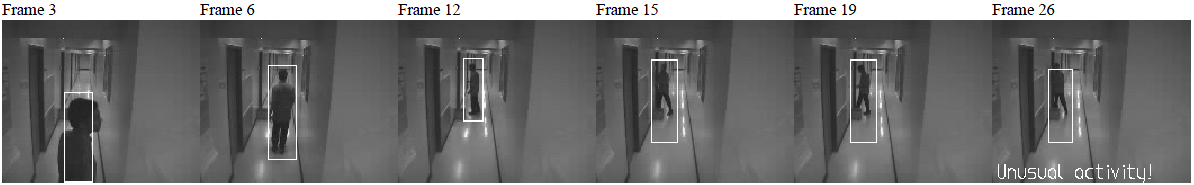
\includegraphics[width=6.1in]{figures/nair-alarm-result.png} 
  \caption[Example of the results of unusual activity
  detection]{Example of the results of unusual activity
  detection. Reprinted from the work of Nair and Clark (2002).}
\label{fig:nair-alarm-result}
\end{figure}

\shortciteA{chan06event} present a HMM-based approach to 
detect rare events in aerial video. An example event in the scene is
shown in Figure \ref{fig:aerial-scene}. They avoid modeling motion
trajectories directly since this is difficult when training data is
lacking. In this paper, they use a continuous HMMs to model the
spatio-temporal relations between objects and uncertainty in
observations. The raw features are object positions, distances between
a source and destination, and velocities. The authors mention that
this requires much training data; so, it is difficult to model and
differentiate the invariant relationships of objects from incidental
activities, such as the object's path between the source and
destination. In order to encode the continuous features to the
relations between objects and uncertainty in observations, they
binarize the features to discrete features by some threshold. The
calculation of binarized feature vector is shown in
Figure \ref{fig:binarized-feature-vector}. They construct a continuous
HMM as shown in Figure \ref{fig:chan-icpr06-hmm}.

\begin{figure}[t]
  \begin{center}
    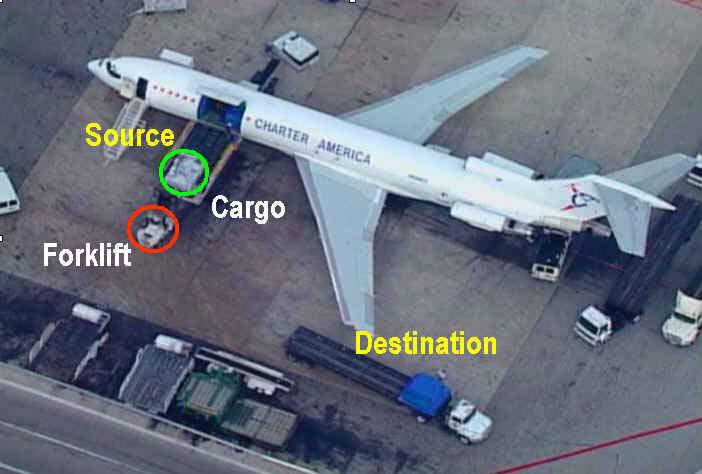
\includegraphics[width=3in]{figures/aerial-scene.jpg} \caption[An
      example event in the aerial scene]{An example event in the
      aerial scene. Reprinted from the work of Chan et al.\
      (2006).} 
    \label{fig:aerial-scene}
  \end{center}
\end{figure}

\begin{figure}[t]
  \begin{center}
    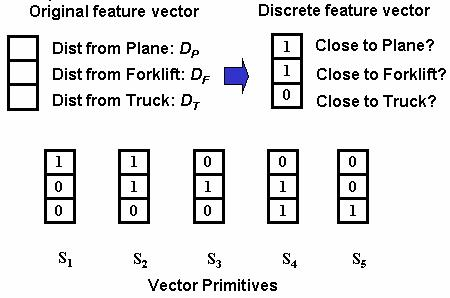
\includegraphics[width=3in]{figures/binarized-feature-vector.jpg}
    \caption[Binarized feature vector]{Binarized feature
    vector. Reprinted from the work of Chan et al.\
    (2006).} \label{fig:binarized-feature-vector}
  \end{center}
\end{figure}

\begin{figure}[t]
  \begin{center}
    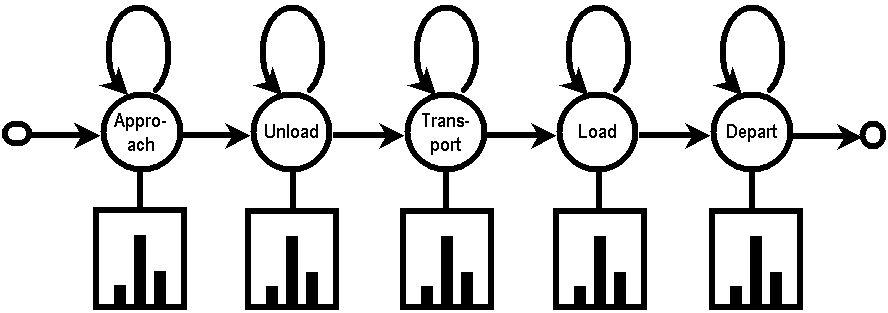
\includegraphics[width=3.5in]{figures/chan-icpr06-hmm.jpg}
    \caption[A continuous HMM with five states that models a complete
    unload and load cycle]{A continuous HMM with five states that
    models a complete unload and load cycle. Reprinted from the work
    of Chan et al.\ (2006).} 
    \label{fig:chan-icpr06-hmm}
  \end{center}
\end{figure}

For modeling a single temporal process, a standard HMM has only one
hidden state and one observation at each time instance. An example of
a HMM is shown in Figure \ref{fig:all-hmms}a. Although HMMs are
powerful, they may be unsuitable for modeling activities when the data
set is very large. They may yield poor models. To address this
problem, HMMs have been extended in a number of ways. The state and
observation space can be factorized using hidden state and multiple
observation variables. The extensions which have been proposed so far
are described as follows.

\shortciteA{brand97chmm} exploit coupled hidden Markov models
(CHMMs) to deal with the causal connections among multiple temporal
processes. In this paper, the author use CHMMs to model two-handed
actions and to classify gestures into 3 categories which are single
whip, brush knee, and cobra. Their experiments presented that CHMMs is
superior compared to conventional HMMs in terms of training speeds,
model likelihoods, and robustness to initial conditions. CHMMs use
fully-connected state space. An example of a CHMM is shown
in~\figurename~\ref{fig:all-hmms}d.

\shortciteA{brand00momchmm} propose a multi-observation and
mixture+counter hidden Markov model (MOMC-HMM). This kind of HMM is
used to factorize the observation space. The authors present that
their framework capable of learning models of office activity and
outdoor traffic. In this paper, they also demonstrate how this
framework can be adapted to infer hidden state from extremely
ambiguous images. For example, it can infer both 3D body pose and
orientation from image sequences of low resolution
silhouettes. \shortciteA{xiang05profiling} also employ this kind of
HMM in their work to learn behavior patterns in a corridor scene, and
detect anomalies such as a person sneaking into the office area
without using an entry card. Figure \ref{fig:xiang-sneaking-result}
shows an example of abnormal behavior patterns. An example of a
MOMC-HMM is shown in Figure \ref{fig:all-hmms}b.

\begin{figure}[t]
  \begin{center}
    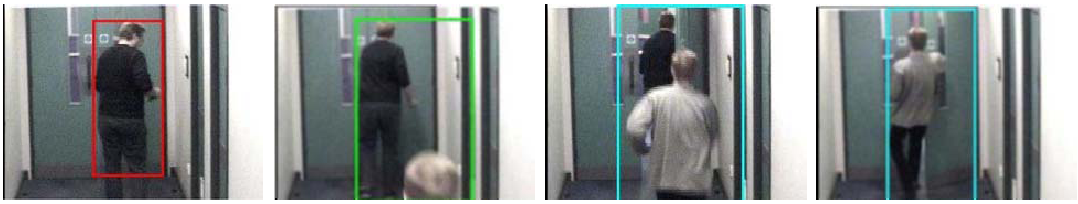
\includegraphics[width=5in]{figures/xiang-sneaking-result.png}    
     \caption[Example of abnormal behavior patterns in a corridor
	scene]{Example of abnormal behavior patterns in a corridor
	scene. A person sneaking into the office area without using an
	entry card.  Reprinted from the work of Xiang and Gong
	(2005).}
    \label{fig:xiang-sneaking-result}
  \end{center}
\end{figure}

\shortciteA{vogler01language} propose parallel hidden Markov models
(PaHMMs). For this kind of HMM, the hidden state space is factorized
into ``state channels" corresponding to multiple independent temporal
processes. Consequently, the channels can be trained completely
independently, and later they can be combined at recognition
time. Since they apply PaHMMs to recognize American sign language
(ASL), it is unnecessary to provide examples of all possible
combinations of phonemes at training time. Thus, ASL can be modeled
independently. Their experiments demonstrate that their approach
outperforms conventional HMMs in dealing with this problem. An example
of a PaHMM of three independent processes is shown
in Figure \ref{fig:all-hmms}c. However, the factorizability
hypothesis is invalid in most cases, particularly when facing the
group or interactive activities.

\shortciteA{gong03activity} propose dynamically multi-linked
hidden Markov model (DML-HMM). The DML-HMM targets connecting a subset
of essential hidden state variables across multiple temporal processes
instead of being fully connected as in the case of a CHMM. The state
transition matrices are factorized using Schawarz's Bayesian
information criterion (BIC) \shortcite{schwarz78bic}. The number of
unnecessary parameters can be reduced for better network structure
discovery. Their experiments in this paper presented that DML-HMM
outperforms a MOMC-HMM, a PaHMM, and a CHMM in modeling group
activities in a cluttered outdoor scene. Figure \ref{fig:gong-results}
presents some of the results of their method. An example of a DML-HMM
is shown in Figure \ref{fig:all-hmms}e.

\begin{figure}[t]
  \centering
  \subfloat[]{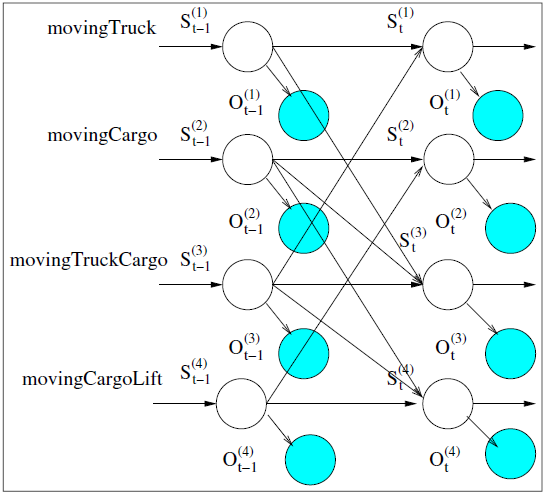
\includegraphics[width=3.5in]{figures/gong-learned-dml-hmm.png}}\\
  \subfloat[]{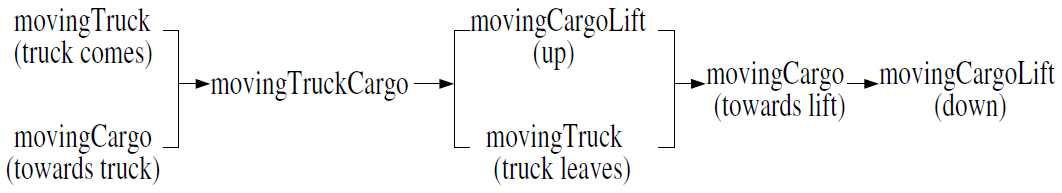
\includegraphics[width=6in]{figures/gong-activity-structure.png}}\\
  \subfloat[]{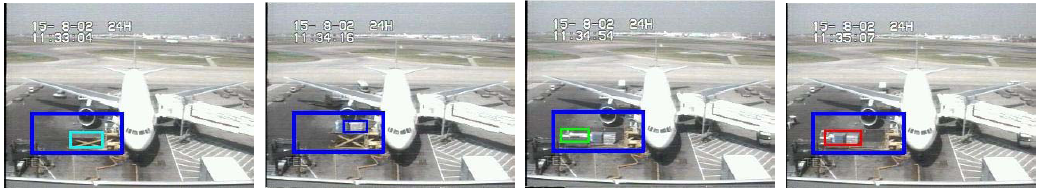
\includegraphics[width=5in]{figures/gong-event-detection.png}}
  \caption[Some results of Gong and Xiang's method]{Some results of Gong and Xiang's method. 
  (a) A learned DML-HMM for modeling four temporal processes corresponding to four classes of events involved in cargo loading/unloading activities. 
  (b) The expected corresponding causal and temporal structure of the activities. 
  (c) Event detection and classification during an aircraft cargo unloading activity. Reprinted from the work of Gong and Xiang (2003).}
  \label{fig:gong-results}
\end{figure}

\begin{figure}[t]
  \centering
  \subfloat[]{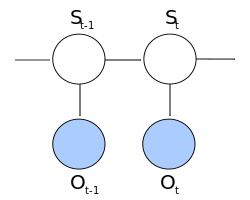
\includegraphics[scale=0.45]{figures/hmm}}
  \hspace{0.1in}
  \subfloat[]{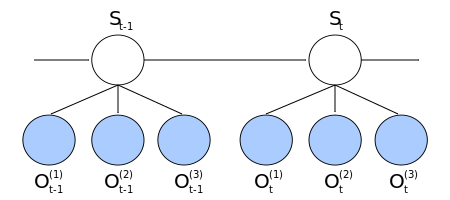
\includegraphics[scale=0.45]{figures/momc-hmm}}\\
  \subfloat[]{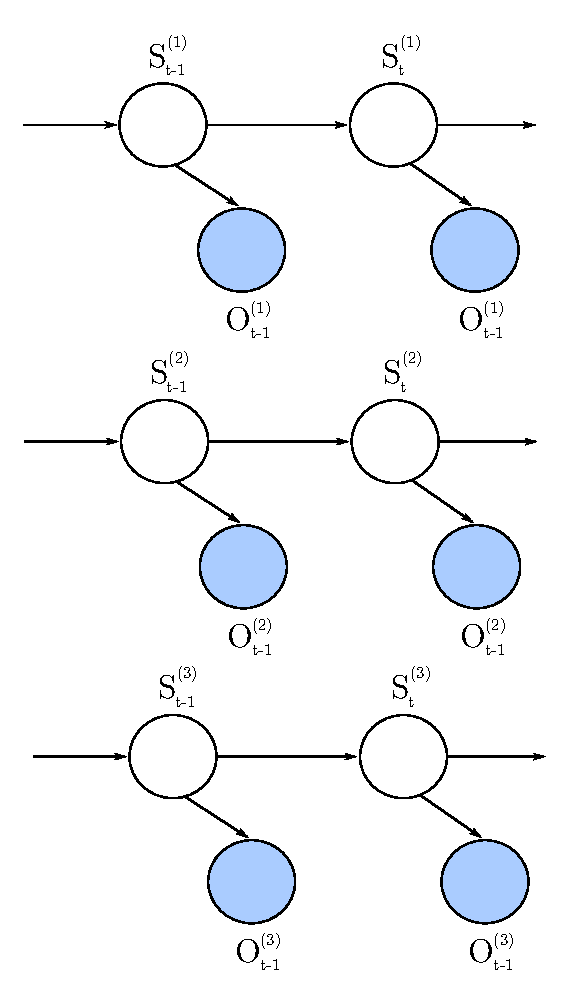
\includegraphics[scale=0.45]{figures/pahmm}}
  \hspace{0.1in}
  \subfloat[]{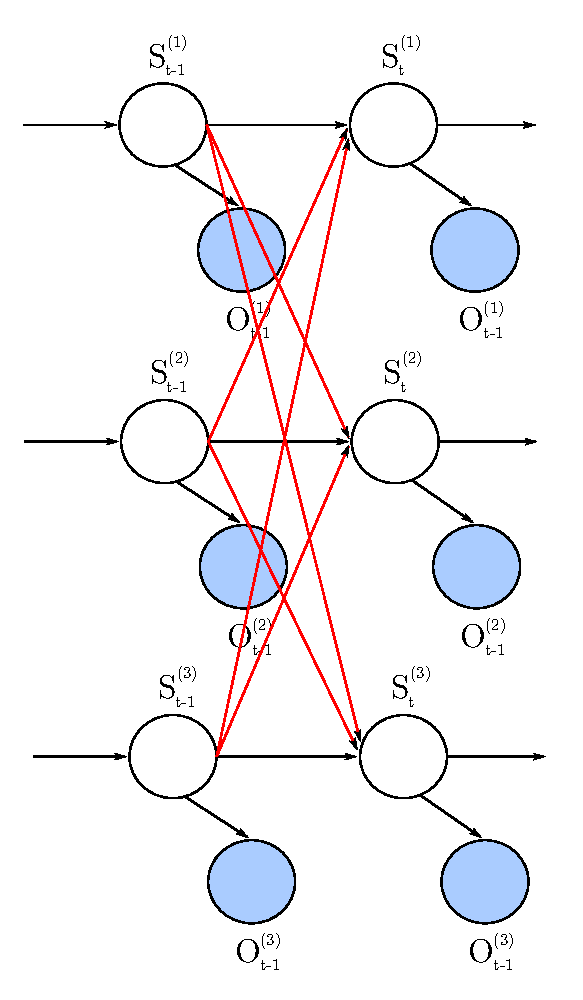
\includegraphics[scale=0.45]{figures/chmm}}
  \hspace{0.1in}
  \subfloat[]{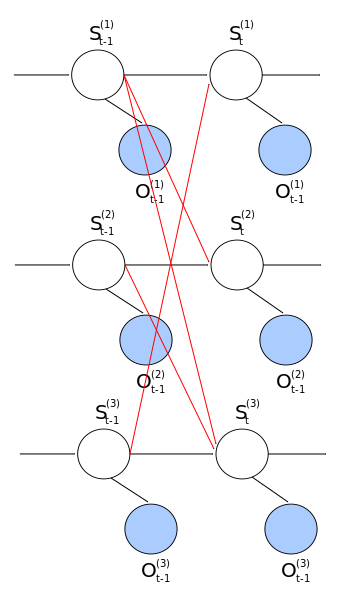
\includegraphics[scale=0.45]{figures/dml-hmm}}
  \caption[Five different types of hidden Markov model]{Five different types of hidden Markov model. The shaded circles represent observation nodes and the white circles represent hidden nodes. 
  (a) HMM. 
  (b) MOMC-HMM. 
  (c) PaHMM. 
  (d) CHMM. 
  (e) DML-HMM.}
  \label{fig:all-hmms}
\end{figure}

Instead of using HMMs, the principal component analysis (PCA) can be
applied in human behavior recognition. \shortciteA{davis98activity}
build an application for human activity recognition using PCA. They
first estimate motion information using an optical flow field. They
track the moving objects using the $W^4$ system, which is a real time
system for tracking people and their body parts. Basically, the system
models the people's movements and tries to answer what, where, and
when they are doing. Also, it provides an appearance model of people
being tracked (who?) through occlusion events. After tracking, the
authors then apply PCA to recognize the activities. In their
experiments, they demonstrate that the method is able to recognize the
similar activities: walking, marching, line-walking, and kicking while
walking.

\shortciteA{masoud03activity} also use PCA technique to recognize
actions. The authors use recursive filtering to extract the features
based on low-level motion features. The technique is appropriate for
real-time application since it is simple and time-efficient. In this
paper, they use five body parts tracking from the work
of \shortciteA{ju96motion}. To make the extracted features more
robust, they normalize the magnitude features since a person wearing
clothes similar to the background will yield low magnitude
features. They also normalize the image size; therefore, the images
will be all of equal dimensions. To classify human actions, the
authors compress the training actions, and compute the distance
between coefficients for a testing action and the coefficients of
every example action, then choose the minimum distance.

In the work of \shortciteA{cao04motion}, they use SVMs to recognize
online human motion. They encode motion information through recursive
filtering and frame grouping. They construct a filtered image using
recursive filtering which is conceptually similar to the motion
history image (MHI) proposed by \shortciteA{davis97mhi}. Then they
classify each filtered image of a video separately using support
vector machines (SVMs). The resulting labels are used to determine the
motion type of the video through majority voting within a sliding
window. Their method shows that it can online classify motions, and
their results also outperform using PCA in offline recognition.

\shortciteA{li06behavior} propose a method based on space-time image
features for automatic behavior modeling and recognition. After the
authors extract the space-time feature representation as described in
Section \ref{literature-review-blob-extraction}, they apply dynamic time 
warping (DTW) to
recognize human behaviors instead of using HMMs.

\shortciteA{du06activity} propose an approach to recognize interaction
activities between two people based on dynamic Bayesian network
(DBN). They divide the work into two phases. The first phase is that
they extracted features of motion, and grouped them into two classes
which are global features and local features. The global features
represent the object's trajectory and the relation between two
objects. The local features represent the motion details such as
aspect ratio of the bounding box. The second phase is that they apply
DBN to recognize activities. To solve some drawbacks from the
conventional HMM such as limited performance to model long-range
process, they add the state duration with a reasonable distribution
into the model.

\shortciteA{wilson00gesture} apply continuous HMMs to recognize human
gestures in an online fashion. They modify the Baum-Welch algorithm to
be able to update parameters at runtime. In this paper, they use a
simple background subtraction to get a silhouette image, and tracked
the body-centric image.

Liu and Cheng (2003)\nocite{liu03face-hmm} apply adaptive continuous
HMM to perform the video-based face recognition. They consider each
frame in a video as one observation. They apply PCA on all face images
to reduce the dimension as well as get feature vectors. They train a
separate HMM on each of the subjects, and used a test sequence to
update the HMM of that subject. They decide to update a model based on
the likelihood difference between the highest and the second highest
likelihood score. The score is large when the recognition is correct,
and it is small when the recognition is incorrect. They update the
model only if the likelihood difference is larger than the pre-defined
threshold. To reestimate the model, only the mean vectors from the
existing HMM are updated since, from their literature, the major
discriminative information of a HMM is retained by the mean vectors.

\shortciteA{zhang05event} propose a method for unusual event
detection using semi-supervised adapted HMMs. They first train an
usual event model and then used the maximum a posteriori (MAP) to
adapt the models as well as model unusual event models. Specifically,
they apply a top-down hierarchical structure and start with only one
node in the tree which represents the usual event model. At each
iteration, they split the usual event model into two models: one
represents an usual event model, and the other one represents an
unusual event model. They adapt both models using MAP. Then they keep
repeating the steps until they obtain the desired number of
iterations. Figure \ref{fig:zhang-algorithm-flow} illustrates the
algorithm flow. Their method does not need explicitly labeled unusual
event data. The experiments illustrate that the proposed method
outperforms both unsupervised and supervised HMM learning fashion.

\begin{figure}[t]
  \begin{center}
    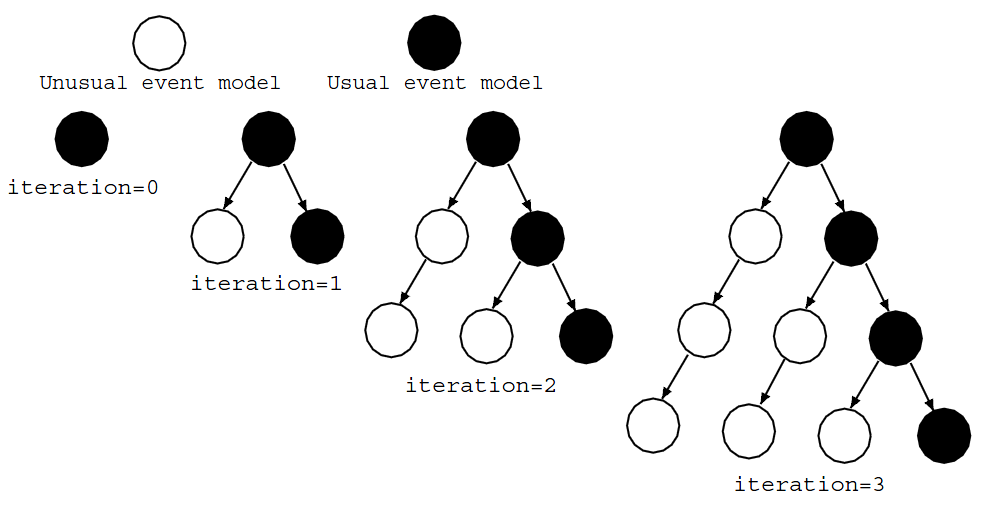
\includegraphics[width=3.5in]{figures/zhang-algorithm-flow.png}
    \caption[The algorithm flow of Zhang et al.'s method]{The
	algorithm flow of Zhang et al.'s method. Two leaf nodes are
	split from the parent usual event node at each
	iteration. Reprinted from the work of Zhang et
	al. (2005).}
    \label{fig:zhang-algorithm-flow}
  \end{center}
\end{figure}

\shortciteA{snoek06event} propose a method for automatically
recognizing usual events on stairs and detecting anomalous events such
as people miss one step or people slip off one step. In their work,
they train a single continuous HMM on all normal sequences and use a
threshold to detect anomalies. They define the threshold by computing
a cost for the validation set and selecting one which minimizes the
summed cost over all of the validation sets. Additionally, in the
experiments, they applied a conditional random field (CRF) to compare
the detection results.

\shortciteA{arsic07behavior} build a video surveillance application
to monitor human behaviors in an airplane situation. They extract
low-level motion features from the complete image based on a simple
difference between images. And they enhance the classification results
by splitting an image into several parts to extract features from the
face area. They apply a pyramidal search with neural network (NN) for
face tracking \shortcite{rowley98face}. Then they use a multi-class
SVM to model and classify behaviors into the pre-defined
classes. Because of unknown start and end state or the length of
motion, their classification is performed by windowing the resulting
time series of features without any overlap.

\shortciteA{andrade06crowd} present an automatic method for modeling
crowd scenes as well as detecting abnormal events. They first model
the background scene and extracted foreground objects. Simultaneously,
they compute the optical flow for the whole scene. Gaussian filter is
used to reduce some noise beforehand. They use the combination of the
foreground mask and flow information to only consider the flow vectors
inside the foreground objects. They encode the motion parameters in a
vector of the form $s = (u, v)$, where $u$ and $v$ are horizontal and
vertical optical flow components. After that they perform PCA on the
optical flow fields of each frame to get a vector representing the
activity pattern. They measure the similarity between video segments
using spectral clustering based on the likelihood given by a
multi-observation HMM (MOHMM), and then they group the segments into
$K$ different classes. They train a MOHHM per class. Then an abnormal
event is detected if the likelihood given by a bank of MOHMM is less
than the detection threshold.

Due to the lack of prior knowledge, poor estimates, violated
assumptions, or insufficient training
data, \shortciteA{bicego09classification} state that the results will
become poor when the improper models are employed. They, therefore,
propose to use the combination of the descriptive strengths of HMMs
with discriminative classifiers to improve the classification results
in those cases. They introduce four major ways of building HMM-induced
vector spaces.

The first vector space is called LL-space (Log-Likelihood space) which
describes how well a sequence is modeled by the given HMM. The second
one is called state-space which describes how often the model passes
through a particular state when observing an observation sequence. The
third one is called trans-space which describes the probability of
passing from the current state $i$ at time $t$ to the next state $j$
at time $(t+1)$. And the fourth one is called emit-space which
describes the characteristic of the model by the sum of emission
probabilities at a given state. The emission probabilities can
represent the most meaning part of a HMM in some applications. Every
feature is able to measure how a specific component of individual HMMs
contributes to the explanation of the observations. Moreover, these
features, ``Component Information", capture the relevant information
extracted from particular components of the models, in relation to the
input observations. For the classification, They construct a new
vector space including these vectors. Then they evaluate their
approach using three discriminative models: naive bayes classifier
(NBC), SVM, and $k$-nearest neighbor ($k$-NN) rule.

\shortciteA{liu09activity} propose a new approach to
distinguish between meaningful and non-meaningful HMM-modeled activity
patterns. The classification is based on a likelihood ratio test
(LRT); however, the proposed method differs from the traditional
LRTs. The authors use the likelihood ratio called pairwise likelihood
ratio (PLR) which is based on each pair of HMMs. Also, this method
does not require to model non-meaningful patterns. Rather than using a
fixed threshold, the authors use the distribution of the likelihood
ratios as the measurement. In this paper, they apply discrete HMMs for
gesture recognition and continuous HMMs for human action recognition.

\subsubsection{Incremental Learning} 
\label{incremental-learning}

Much research has started to focus on applying the incremental
learning techniques to improve real-time surveillance systems. In this
dissertation, I focus on only the use of hidden Markov models
(HMMs). One major problem of applying HMMs is that HMMs need excessive
computing resources in the training process if we have large amount of
data. Additionally, we are required to store the whole data together
with the new data in order to retrain the models. This is obviously
unsuitable for the real-time applications, especially the video
surveillance systems. It is impractical to store the whole video data
since most surveillance systems record video all the time, and the
disk space is limited. Even though we store only the video in which
motion is detected, it still does not solve the problem.

Since the traditional HMM training process demands lots of computing
resources, and it requires storing large databases of training
data. This makes it inefficient for practical surveillance
systems. Using the sufficient statistics and incrementally update the
model parameters seem to be a promising solution to overcome these
problems.

For HMM parameters' estimation, the expectation-maximization (EM)
algorithm \shortcite{dempster77em} can be applied. One well-known
algorithm for this estimation is called the Baum-Welch (BW) algorithm
which is a generalized expectation-maximization (GEM) algorithm. This
algorithm computes maximum likelihood estimates and maximum a
posteriori estimates for the transition and emission probabilities of
HMMs, given only emissions. In this section, I review three
incremental HMM learning algorithms including the incremental
Baum-Welch (BW) algorithm, the incremental maximum-likelihood (IML)
algorithm, and the ensemble training (ET) algorithm.

\shortciteA{stenger01topology} first propose the incremental
Baum-Welch (IBW) algorithm for modeling continuous observations. This
algorithm is a straight-forward adaptation of the original BW
algorithm to incremental
learning. Later, \shortciteA{larrahondo05incremental} adapt the
algorithm to model discrete observations.

The IBW algorithm performs a partial E-step using a single observation
sequence and a M-step for each time step $t$. This means that the
transition and emission matrices of a HMM are updated at each time
step $t$, given the previous model $\lambda_{t-1}$ and a block of data
$D_t$, where $D_t$ is composed of a single observation
sequence. Stenger et al.\ estimated the transition probability, $\bar
a_{ij}^t$, at the current time $t$ as:
\[
  \bar a_{ij}^t  = \frac{{\bar a_{ij}^{t - 1} (\sum\limits_{t' = 1}^{t - 2} 
  {\gamma _{t'} (i)} ) + \xi _{t - 1} (i,j)}}{{\sum\limits_{t' = 1}^{t - 1} 
  {\gamma _{t'} (i)} }}
\]
and the emission probability, $\bar b_j^t(k)$, is defined as:
\[
  \bar b_j^t(k)  = \frac{{\bar b_j^{t - 1} (k)(\sum\limits_{t' = 1}^{t - 1} 
  {\gamma _{t'} (j)} ) + \psi (t,j,k)}}{{\sum\limits_{t' = 1}^t {\gamma _{t'} 
  (j)} }}
\]
where $\psi (t,j,k)$ is an auxiliary function defined as:
\[
  \psi (t,j,k) = \left\{ \begin{array}{l}
  0\quad \quad \;\;{\rm if}\;O_t  \ne v_k  \\ 
  \gamma _t (j)\quad {\rm otherwise} \\ 
  \end{array} \right.
\]
As seen above, the equations update the parameters by taking into
account the sufficient statistics that is stored in $\gamma _{t'} (i)$
from $t'=1,\ldots,t$. Although the estimate equations use a single
observation sequence to update $\lambda_{t-1}$, the sufficient
statistics represent the information computed for all of the observed
data.

\shortciteA{gotoh96incremental} propose the incremental
maximum-likelihood (IML) algorithm, and demonstrate that it performs
faster convergence than the Baum-Welch (BW) algorithm as well as
reduces the memory requirements. The authors store the sufficient
statistics, and use them to incrementally update the model
parameters. They use the idea from the work of \shortciteA{neal93em}
who first apply the concept of using sufficient statistics for the EM
algorithm. Moreover, Neal and Hinton theoretically justify the
incremental versions of the EM algorithm using sufficient statistics,
and prove that the likelihood increases
monotonically. \shortciteA{xiang08incremental} also apply the concept
of sufficient statistics to learn activities incrementally for online
abnormality detection in a visual surveillance scene.

In order to perform the proposed IML
algorithm, \shortciteA{gotoh96incremental} separated the training data
into smaller subsets (blocks). In the E-step, Gotoh and Silverman
calculate the sufficient statistics $S$ of each block, and accumulate
them to use in the M-step. The algorithm works according to the
following steps:

\begin{enumerate}
  \item Initialize the sufficient statistics $S$ to zero.
  \item In the E-step:
  \begin{itemize}
    \item Compute the sufficient statistics of one subset.
    \item Set the sufficient statistics for the whole data set by accumulating them.
  \end{itemize}
  \item In the M-step:
  \begin{itemize}
    \item Update the HMM parameters according to the accumulated sufficient statistics.
  \end{itemize}
\end{enumerate}

In addition to using the blocks of data, we can adapt the IML
algorithm to calculate the sufficient statistics of only one
observation sequence. Therefore, we will get the re-estimation formula
as follows:
\[
	\pi _i  = \frac{{\gamma _{Z,1} (i) + \sum\limits_{z = 1}^{Z - 1} 
	{\gamma_{z,1} (i)} }}{Z}
\]
\[
	a_{i,j}  = \frac{{\sum\limits_{t = 1}^{T - 1} {\xi _{Z,t} (i,j)}  + 
	\sum\limits_{z = 1}^{Z - 1}{\sum\limits_{t = 1}^{T - 1}{\xi _{z,t}(i,j)} } 
	}}{{\sum\limits_{t = 1}^{T - 1}{\gamma _{Z,t}(i)}+\sum\limits_{z = 1}^{Z-1} 
	{\sum\limits_{t = 1}^{T - 1} {\gamma _{z,t} (i)} } }}
\]
\[
	b_j (k) = \frac{{\sum\limits_{\mathop {t = 1}\limits_{s.t.O_{Z,t}=v_k } }^T 
	{\gamma _{Z,t} (j)}  + \sum\limits_{z = 1}^{Z - 1}{\sum\limits_{\mathop 
	{t=1}\limits_{s.t.O_{z,t}=v_k}}^{T - 1}{\gamma _{z,t} (j)}} 
	}}{{\sum\limits_{t = 1}^T {\gamma _{Z,t} (j)}  + \sum\limits_{z = 1}^{Z - 1} 
	{\sum\limits_{t = 1}^T {\gamma _{z,t} (j)} } }}
\]
where $Z$ is the number of observation sequences. From the above
equation, we store the sufficient statistics of all of the sequences
in the past. And accumulate them into the current sufficient
statistics at the current time step.

For each iteration, we just add the sufficient statistics in the past
to the new one. Once we finish updating the model, we replace the old
sufficient statistics. However, \shortciteA{nowlan91incremental}
propose an incremental approach which does not require remembering
$\vec{S}_z$ for all $z$ by simply adding the new sufficient statistics
in with a forgetting factor in the following way:
\[
	\vec{S}^{new} = \alpha \vec{S}^{old} + \vec{S}_z
\]
where $\alpha$ is the forgetting factor.

\shortciteA{cavalin08incremental} adapt the ensemble training (ET)
algorithm which is first propose in the work
of \shortciteA{mackay97hmm} to the incremental learning problem. This
algorithm has never been used in incremental learning setting. Cavalin
et al.\ claimed that it is easy to adapt to this kind of setting since
the parameters of the final HMM are computed for each observation
sequence independently.

To perform the ET algorithm, suppose that we have $K$ observation
sequences for training, and for each sequence, we estimate one model
$\parms_k$ by ET which results in the formation of $K$ independent
model. Then we merge these $K$ models into one final model in the
following way:
\[
	\bar a_{ij}  = \frac{{\sum\nolimits_k {W_k a_{ij}^k } }}{{\sum\nolimits_k 
	{W_k } }}
\]
\[
	\bar b_{ij}  = \frac{{\sum\nolimits_k {W_k b_{ij}^k } }}{{\sum\nolimits_k 
	{W_k } }}
\]
\[
	\bar \pi _i  = \frac{{\sum\nolimits_k {W_k \pi _i^k } }}{{\sum\nolimits_k 
	{W_k } }}
\]
where $W_t$ is a weight for an observation sequence at the current
time $t$. Clearly, each HMM must have the same number of states and
observation symbols.

We store a current HMM $\parms_{t-1}$ which corresponds to all data up
to the time step $t-1$. We reestimate the new model $\parms_t$ when
new data is available by consider only $\parms_{t-1}$ and
$\parms_t$. One important aspect to assure that the old information is
stored in $\parms_t$ is the weights. Thus, we accumulate both
$W_{t-1}$ and $W_{t'}$ into $W_{t}$. Therefore, we will get the
re-estimation equation for the weights as follows:
\[
	\bar a_{ij}^t  = \frac{{W_{t - 1} a_{ij}^{t - 1} + W_{t'} a_{ij}^{t'}}}
	{{W_{t - 1}  + W_t }}
\]
\[
	\bar b_{ij}^t  = \frac{{W_{t - 1} b_{ij}^{t - 1} + W_{t'} b_{ij}^{t'}}}
	{{W_{t - 1}  + W_t }}
\]
\[
	\bar \pi _{ij}^t  = \frac{{W_{t - 1} \pi _i^{t - 1} + W_{t'} \pi _i^{t'}}}
	{{W_{t - 1}  + W_t }}
\]
\[
	W_t  = W_{t - 1} + W_{t'} 
\]
For the initial models, the authors used the models with equal values
for all parameters. Also, the number of states and tokens have to be
fixed due to the appropriateness of mixing them later.

However, the incremental learning algorithms, including the IBW
algorithm, the IML algorithm, and the ET algorithm, need to manually
or experimentally fix the model structure in advance. Therefore, this
is unsuitable for real-world autonomous systems.

\subsubsection{Online Model Topology Adaptation} 
\label{topology-adaptation}

In addition to incremental learning with a fixed topology, a dynamic
mechanism to learn and update the model topology is also important to
real-time surveillance applications. For HMMs, most of the existing
works in the literature need to define the number of states and tokens
beforehand. This may cause some problems since most real-world
applications use a stationary assumption on the model
parameters. However, most of them are usually non-stationary in
nature. There are two possible ways to automatically estimate the
optimal number of states for HMM topology which are state
splitting \shortcite{li99pattern,stenger01topology,siddiqi07topology}
and state merging \shortcite{stolcke93topology}.

\shortciteA{stolcke93topology} present an approach for learning the
HMM topology using Bayesian model merging. The authors use the
Bayesian posterior probability to determine when to stop merging. The
algorithm starts with a HMM that produces exactly the input
sequences. Each sequence is represented by a unique path with one
state per observation. Then the start state is introduced to connect
to all of the paths and the transition probability is uniformly
distributed. This also means that the most specific model is
constructed for the training data. Given the current model, the
merging process selects a pair of states for merging that maximizes
the probability of the candidate model given the observations. The
process stops when the posterior probability decreases.

\shortciteA{li99pattern} optimize the HMM topology by splitting the
state if it has the largest variance, and merging the two states if
they have the closest means. The authors train the model candidates
using the BW algorithm on the entire HMM, then selected the candidate
with higher likelihood. When the candidates are worse then the
original model, the process stops.

\shortciteA{stenger01topology} present a framework for HMM topology
and parameter estimations in an online fashion. They explore the use
of state splitting algorithm with various model selection criteria
including a chi-square goodness of fit test, a cross-validation
criterion, and a minimum description length (MDL) stopping
criterion \shortcite{rissanen98mdl}. In this paper, the authors apply
their algorithms to solve the background modeling problem. Generally,
their state splitting algorithm can be described as follows.

\begin{enumerate}
  \item Initialize a HMM with one state.
  \item Use the BW algorithm to train the data set.
  \item Compute the likelihood of the test set given the trained model.
  \item If the likelihood decreases, stop.
  \item Select a split candidate which satisfies the defined criteria, then split the state.
  \item Go to step 2.
\end{enumerate}

Their experiments demonstrate that using MDL stopping criterion yields
compact HMM topologies and fair accuracy compared to the chi-square
goodness of fit test and the cross-validation.

\shortciteA{siddiqi07topology} propose a novel approach for HMM
model selection and learning. The idea is to incrementally increase
the number of states while learning HMM parameters. They construct the
candidate models by splitting the existing states and optimizing the
parameters, and then select the optimal model. In this paper, they use
the Bayesian information criterion (BIC) \shortcite{schwarz78bic} to
determine when to stop splitting the states.

\subsection{Summary}

Recently, lots of research have started to focus on developing an
algorithm capable of recognizing activites as well as detecting
abnormal ones in a given scene. One limitation of most of the work is
that the number of ``normal" behavior patterns need to be known
beforehand. Another limitation is that most of the works learn in
batch mode, and create separate models for each distinct class of
behavior.

Using the batch training is known to be robust, but it has some
disadvantages. Apart from requiring to store the large training data
set and requiring excessive computing resources, the data
representation may not be good enough to the general problem. As a
real time application such as a video surveillance system records
video over time, it is unsuitable to retrain every time when we have a
new data.

There are some interesting techiniques I can apply in this
dissertation. One technique is to use the combination of the
descriptive strengths of HMMs with discriminative classifiers to
improve the classification when we have insufficient data or lack of
prior knowledge. This technique is proposed
by \shortciteA{bicego09classification}. Another technique proposed
by \shortciteA{cao04motion} is to apply SVMs with a sliding window
to deal with sequential data. For the online training technique, I
will apply the work of \shortciteA{gotoh96incremental} on incremental
learning and the work of \shortciteA{stenger01topology} on model
topology adaptation.

%\section{Related Algorithms}
%
%The related algorithms are as follows.
%
%\subsection{Bayesian Probability}
%
%Bayesian probability \shortcite{huang94inference} is one of the most
%popular methods to interpret the concept of probability. It enables
%reasoning with uncertain statements. To evaluate the probability of a
%hypothesis, one gives some prior probability which will be updated
%when the new relevant data come.  Given the data, the probability of a
%hypothesis is proportional to the product of the likelihood times the
%prior probability. The likelihood takes the effect of data into
%account. And the prior probability gives the probability of the
%hypothesis before the data are observed. The Bayesian inference uses
%Bayes' formula which is defined as:
%\[
%  P(A \mid B) = \frac{{P(B \mid A)P(A)}}{{P(B)}},
%\]
%where $P(B)$ is the prior probability, $P(A)$ is the marginal
%probability, $P(B \mid A)$ is the conditional probability or is called
%the likelihood, and $P(A \mid B)$ is the posterior probability.
%
%\subsection{Bayesian Belief Network}
%
%Bayesian Belief Network (BBN; Pearl, 1988) \nocite{pearl88reasoning}
%is a powerful tool for modeling, and enables us to model and reason
%about uncertainty. It is being increasingly used in a wide variety of
%domains where automated reasoning is needed. BBN provides a rich
%representation of directed graph along with a set of conditional
%probability tables. The graph consists of nodes and arcs. An example
%of a Bayesian belief network is shown in Figure
%\ref{fig:bayes-net}. The nodes represent discrete or continuous
%variables, and the arcs represent causal or influential relationships
%between variables. BBN is mainly used in situations where the
%statistical inference is required. Users may know some evidence or are
%observing some event. And they may want to know the probabilities of
%other unobserved events. Therefore, the probability calculus and
%Bayes' theorem \shortcite{huang94inference} can be used to infer and
%update the values of all the other probabilities in the BBN. This is
%called propagation.
%
%\begin{figure}[t]
%  \centering
%  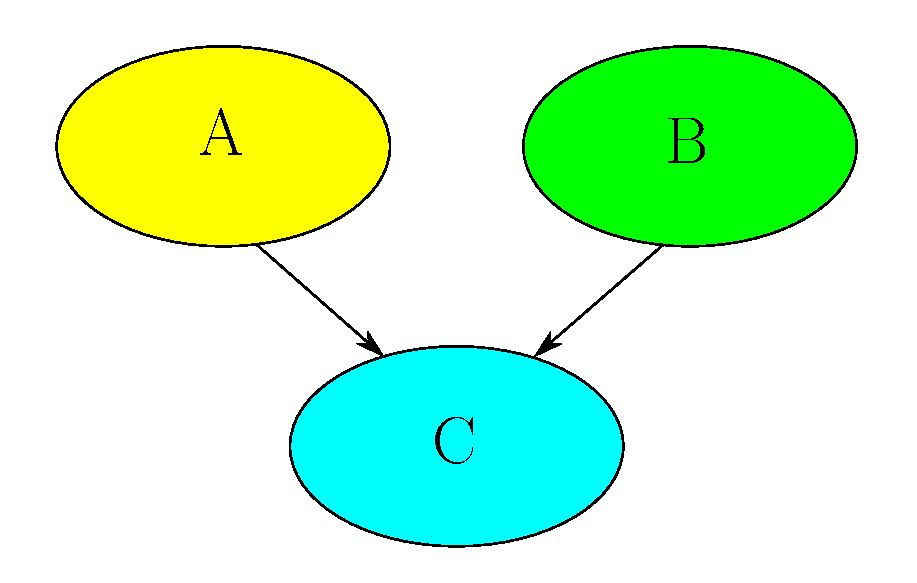
\includegraphics[width=1.5in]{figures/bayes-net}
%  \caption[Example of a Bayesian belief network]{Example of a Bayesian
%    belief network.}
%  \label{fig:bayes-net}
%\end{figure}
%
%\subsection{Principal Component Analysis}
%
%Principal Component Analysis (PCA; Wikipedia, 2010) \nocite{wiki10pca}
%is a useful statistical technique that has been applied in many fields
%such as face recognition. It is used as a tool for analyzing data and
%finding patterns in high dimensional data. As well, it is a common
%technique to reduce the number of dimensions. In other words, PCA
%mathematically transforms a number of possible correlated variables
%into a smaller number of uncorrelated variables called principal
%components.
%
%\subsection{Hidden Markov Model}
%
%The hidden Markov model (HMM; Rabiner, 1998) \nocite{rabiner98hmm} is
%a generative probabilistic model, and it is also a stochastic process
%in which the system being modeled is assumed to be a Markov process
%with unobservable states. HMM contains a finite set of states. The
%state cannot be observed directly, but the output. Each state is
%associated with a probability distribution over the possible
%observations. Therefore, a HMM can produce the observation sequence
%given the information about the state sequence. A HMM has the
%following components:
%
%\begin{enumerate}
%  \item $N$ is the number of states of the model. The set of states is
%    defined as $S = \{ S_1, \ldots, S_N \}$ and the state at time $t$
%    is defined as $q_t$.
%
%  \item $M$ is the number of observation symbols of the model. The set
%    of observation symbols is defined as $V = \{ v_1, \ldots, v_M \}$.
%
%  \item The transition probability is defined as $\mat{A} = \{ a_{ij}
%    \}$, where $a_{ij} = P(q_{t+1} = S_j\mid q_t = S_i)$ is the
%    probability of being in state $S_j$ at time $t+1$ given we were in
%    state $S_i$ at time $t$.
%
%  \item The emission probability in state $j$ is defined as
%    $\mat{B}=\{b_j(k) \}$, where $b_j(k) = P(v_k\;{\rm at}\;t \mid q_t
%    = S_j)$ is the probability of being observing symbol $v_k$ given
%    we are in state $S_j$.
%
%  \item The initial probability is defined as $\vec{\pi} = \{ \pi _i
%    \}$, where $\pi_i = P(q_1 = S_i)$ is the probability of being in
%    state $i$ at time $t$.
%
%  \item The observation sequence is defined as $O = \{O_1, \ldots, O_T
%    \}$ and $O_t$ is the observation symbol at time $t$
%\end{enumerate}
%
%The compact notation to represent as HMM is $\parms = \{\mat{A},
%\mat{B}, \vec{\pi}\}$.
%
%\subsection{Conditional Random Field}
%
%A Conditional Random Field (CRF; Lafferty et al., 2001)
%\nocite{lafferty01crf} is an undirected graph which is mostly used for
%labeling the sequential data. CRF is widely applied in natural
%language processing (NLP). The difference between CRF and HMM is that
%HMM is generative and models the joint probability distribution while
%CRF is discriminative and models the conditional probability
%distribution of interest. One advantage of CRF is that it conditions
%on the entire observation sequences, and it does not need the
%assumptions of independence between observations. The set of features
%that can be incorporated into the model is expanded by conditioning on
%the observations without any violations to the assumptions.
%
%\subsection{Support Vector Machine}
%
%Support Vector Machine (SVM; Vapnik, 1995) \nocite{vapnik95svm} is a
%machine learning algorithm that learns by example to assign classes to
%objects. SVM becomes very popular in a wide variety of many
%applications such as hand writing recognition, face recognition, and
%especially for pattern classification based applications. Given a set
%of training examples, SVM constructs a hyperplane or set of
%hyperplanes in high dimensional space for classification or
%regression. Then the algorithm maximizes the distance of the
%hyperplane to the nearest training data points of any class to achieve
%a good separation. New data will be then classified into a class based
%on which side of the hyperplane they fall on.
%
%\subsection{Dynamic Time Warping}
%
%Dynamic Time Waring (DTW; Sakoe, 1978) \nocite{sakoe78dtw} is an
%algorithm for finding the similarity between two sequences which may
%vary in time or speed. Generally, DTW provides an optimal match
%between two given sequences with some restrictions. The algorithm
%warps each of the sequences non-linearly in the time dimension to
%compute the similarity. DTW has been widely applied in many
%applications regarding video, audio, and graphics. Actually, any data
%which can be turned into a linear representation can be analyzed using
%DTW. Most applications that apply DTW have been automatic speech
%recognition to deal with different speaking speeds. In addition, DTW
%can be applied in searching the similar activity patterns. For
%instance, a person is walking slowly and another person is walking
%more quickly; so, the similarity in this walking pattern can be
%detected.
%
%\subsection{Hierarchical Clustering}
%
%Hierarchical Clustering (HC; Hastie et al., 2009) \nocite{hastie09hc}
%is a clustering method that builds a hierarchy of clusters. There are
%two methods for HC which are the agglomerative approach and the
%divisive approach. For the agglomerative approach (bottom-up
%approach), the algorithm starts from the bottom where one cluster
%represents one object, and then it goes up through merging of the two
%closest clusters. The process is iterated until all clusters are
%aggregated into a single cluster. For the divisive approach (top-down
%approach), the algorithm starts from a single cluster containing all
%objects, and then it splits the cluster into two recursively until
%each cluster contains a single object.
